\documentclass[submission, copyright,creativecommons,sharealike,noncommercial]{eptcs}
\providecommand{\event}{Swarm community}
%
%
%%%%%%%%%%%%%%%%%%%%%%%%%%%%%%%%%%%%%%%
%%%%%%%%%% TITLE AND AUTHORS %%%%%%%%%%
%%%%%%%%%%%%%%%%%%%%%%%%%%%%%%%%%%%%%%%
\title{Liquid Democracy Voting System for the Swarm Platform}
\author{Fabrizio Romano Genovese
	\institute{Swarm Team}
	\institute{Quantum Group \\ University of Oxford}
	\email{fabrizio@swarm.fund}
\and
Jelle Herold
	\institute{Swarm Team}
	\email{jelle@swarm.fund}
}
\def\titlerunning{Voting System for the Swarm Platform}
\def\authorrunning{F.R.Genovese \& J. Herold}
\usepackage{wrapfig}
%
%
%%%%%%%%%%%%%%%%%%%%%%%%%%%%%%%%%%%%%%%
%%%%%%%%%%%%%% PACKAGES %%%%%%%%%%%%%%%
%%%%%%%%%%%%%%%%%%%%%%%%%%%%%%%%%%%%%%%
%% Display Graphics
\usepackage{graphicx}
%
%% Dynamic spacing for macros
\usepackage{xspace}
%
%% Define 'definition' environment
\usepackage{amsmath}
\usepackage{amsfonts}
\usepackage{thmtools}
\declaretheorem[
style=definition, 
name=Definition
]{definition}
%
%% Gothic letters to define the range set
\usepackage{eufrak}
%
%
%%%%%%%%%%%%%%%%%%%%%%%%%%%%%%%%%%%%%%%
%%%%%%%%%%%%%%% MACROS %%%%%%%%%%%%%%%%
%%%%%%%%%%%%%%%%%%%%%%%%%%%%%%%%%%%%%%%
%% Candidates and range sets
\newcommand{\candidates}{\ensuremath{\mathcal{C}} \xspace} 
\newcommand{\range}{\ensuremath{\mathfrak{R}}\xspace}
%
%% Contract names
\newcommand{\Candidates}{\textbf{CANDIDATES}\xspace} 
\newcommand{\Choices}{\textbf{CHOICES}\xspace} 
\newcommand{\Vote}{\textbf{VOTE}\xspace}
\newcommand{\Reputation}{\textbf{REPUTATION}\xspace} 
%%%%%%%%%%%%%%%%%%%%%%%%%%%%%%%%%%%%%%%
%%%%%%%%%%%%%%%%%%%%%%%%%%%%%%%%%%%%%%%
%%%%%%%%%%%%%%%%%%%%%%%%%%%%%%%%%%%%%%%
%
%
\begin{document}

%	\bibliographystyle{eptcs}
	
	\maketitle

	\begin{abstract}
		Here we highlight how the voting system is going to work. We will start briefly reviewing existent solutions, we will proceed sketching the general idea for the voting system on the Swarm Platform and, finally, we will dive into details producing a working algorithm.
	\end{abstract}

\section{Pre-existent solutions}\label{sec:Pre-existent solutions}
	The need to define a voting system is not a new problem for the blockchain community. For instance, if some altcoin is going to hard fork, the developing team will often ask the user base to express a preference about which branch to adopt. It is obvious, then, that in a situation like this some kind of procedure has to be devised to allow people to express this preference, that is, to allow people to vote.
	
	One of the most common ways to deal with this problem is by issuing some voting tokens and creating two addresses that stand for \emph{yes} and \emph{no}. Every user receives a number of tokens equal to the number of coins owned and sends them to one of these two addresses, expressing a preference.
	
	Albeit very simple to implement, this method has many fundamental flaws that make it not suitable for a system that has democracy -- and hence voting -- at its center:
	\begin{enumerate}	
		\item First of all, a voting procedure like the one highlighted above is very similar to majority voting and, as such, it is cursed by many downsides. One of the biggest achievement of social choice theory is proving that many of the voting systems that people intuitively consider ``fair'' are not fair at all, meaning that they are prone to any sort of manipulation [] or can even be dictatorial []. Voting with tokens as stated above is no exception. 
		%
		\item In the very same moment someone votes, the tokens are transferred to the address expressing a preference, and can be publicly seen. This means that a sufficiently skilled user is able to see in real time who is winning the vote. This exposes the system because gives away data that can be employed for any kind of manipulation.
		%
		\item ``Real'' tokens can be exchanged while the voting ones remain in one's wallet. This means that voting power is not really related to the quantity of money one owns: In a transaction happening after the voting tokens are issued, the person receiving the real tokens has no voting power whatsoever while, on the other hand, the other person retains the voting power without having real stake.
		
		For instance, someone with a lot of real tokens could sell them all, and then use the voting tokens he retained to vote for a very bad decision for the platform. At this point the tokens he just sold will be depreciated because of this bad decision and the person will be able to buy them back at a fraction of the price, making a profit. 
		
		This means that a very powerful user on the platform could exploit the democratic infrastructure to make direct profits.
		%
		\item There is no reputation system. This means that a user voting power is only proportional to the amount of coins owned. A lot of important parameters (how active that user is on the platform, how much money one moves every month, how much that user helped with proposals, \dots) are completely disregarded.
		%
		\item Vote delegation is messy, or even not impossible.
	\end{enumerate}
%
	For these reasons we deemed necessary to steer away from all the pre-existing solutions and design an ad-hoc voting environment that is reasonably fair (according to social choice theory) and suitable to be used on a daily basis.
%
%
\section{Range Voting}\label{sec:Range voting}
	\begin{wrapfigure}{r}{0.5\textwidth}
		\vspace{-10pt}
		\begin{center}
			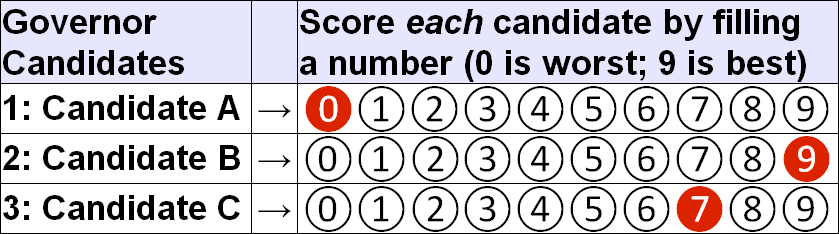
\includegraphics[width=0.48\textwidth]{Voting_Ballot.png}
		\end{center}
		\vspace{-15pt}
		\caption{Range voting ballot [source: Wikipedia]}
		\vspace{-5pt}
	\end{wrapfigure}
%
	The voting method we choose for the platform is \emph{range voting}. Range voting is one of the fairest voting systems available. In particular, being it a \emph{cardinal} and not an \emph{ordinal}\footnote{These are technical terms of voting theory. You can safely ignore them if you don't know what they mean.} voting system, many of the mathematical results about unfairness and dictatorship, such as [], do not apply.
	
	In range voting, each voter can rank each choice giving a score, for instance from $0$ to $10$, where $0$ stands for ``I absolutely don't like this choice'' and $10$ stands for ``I absolutely love it'' (see for instance Figure~[]). When the voting closes, the scores for each choice are summed, and the choice with more points is the one that wins.
	
	There are many groups that actively advocate for range voting to be adopted in electoral laws all around the world, and in addition to this range voting is also considerd one of the best voting procedure available in company administration (see, for instance [][]). 
	
	To conclude, in choosing the right voting procedure for the Swarm platform we consulted decades of research and study on voting systems to find the best alternative available, and we are fairly convinced that range voting is the one.
%
%	
\subsection{Reputation}\label{subsec:Reputation}
%
	Taking into account ``modifiers of the voting power'' is also very easy when one adopts range voting. Let's suppose, for instance, that we want to have a system where the power of a voter is proportional to the number of coins he owns. If voter $A$ owns $n$ coins, then it will be sufficient to multiply by $n$ all the scores that $A$ gives to each candidate. So, for instance, if $A$ owns $10$ coins and ranks a candidate with a score of $5$, that candidate will receive $10*5=50$ points.
	
	To be precise, we want to take into account more parameters than just the quantity of money a voter has to determine the voting power, but now we do not need any new concept to do this. For each user $A$, we will just calculate a multiplier, denoted with $\rho_A$ and called \emph{reputation of $A$}, considering all the parameters that we deem relevant. Again, everything we will need to do to make $A$'s votes proportional to his reputation is to multiply all the scores that $A$ assigns by $\rho_A$.
%
%
\subsection{Drafts}\label{subsec:Drafts}
%
	Clearly, it may happen that a vote leads to a draft. In range voting this means that there are two or more candidates at the top of the points list having the same score. For instance, imagine we have to elect three people for a company board and there are ten candidates, with their ranking in terms of points as follows:
	\begin{center}
	\begin{tabular}{| l | r |}
		\hline
		\textbf{Candidate} & \textbf{Points}\\
		\hline			
		Candidate 7 & 247\\
		Candidate 2 & 133\\
		Candidate 5 & 102\\
		Candidate 8 & 102\\
		Candidate 10 & 84\\
		Candidate 1 & 58\\
		Candidate 6 & 37\\
		Candidate 3 & 29\\
		Candidate 9 & 14\\
		Candidate 4 & 3\\
		\hline  
	\end{tabular}
	\end{center}
%
	Since we are selecting only three members for the board, we have to pick the three best performing candidates. This obviously includes candidates $7$ and $2$, but then we are stucked because candidate $5$ and $8$ have the same amount of points. So who who among the two do we choose?
	
	In classic range voting, at this point, another voting round is held. We discussed at length about implementing such a system for Swarm, and we decided that it wasn't a good idea, first because it puts much more stress and responsibility on users that will have to vote two times, and second because it would make the actual code much more complicated and difficult to audit. So we went for a system in which no second round is needed, as follows:
	\begin{itemize}
		\item If there is an ex-aequo situation, we will prefer the candidate with the highest reputation.
		\item If this doesn't solve the problem (there are multiple winning candidates with the same reputation), then the choice is pseudorandom.
	\end{itemize}
%
%
\section{The voting algorithm -- Intuitive explanation}\label{sec:Voting intuitive}
%
\subsubsection{Desiderata}\label{subsubsec:Desiderata}
	Now that we know what we want, we have to implement it. There are some fundamental desiderata we require:
	\begin{itemize}
		\item The voting should be transparent. This means that all the relevant information should be stored on the blockchain, and every user should be able to calculate the vote outcome independently, as well as to check that is preference was correctly submitted.
		%
		\item The voting should be encrypted. As we said in Section~\ref{sec:Pre-existent solutions}, one problem of voting on the blockchain is that people can know who is winning before the voting window closes. To avoid such a situation, every vote should be encrypted and readable only when the voting window closes.
		%
		\item Being an active member of the Swarm democracy should increase a member reputation. Swarm values participation, and it makes sense that ``the more you vote, the more your vote becomes powerful''. This is also a way to value the experience and time spent on the platform.
		%
		\item The reputation should also be proportional to the amount of Swarm tokens owned. More specifically, if one owns zero Swarm tokens then his voting power should be zero (meaning that has no influence whatsoever).
		%
		\item Delegation must be possible. The word ``delegation'' is actually the reason why we talk about \emph{liquid democracy} and not just about \emph{deocracy}. The idea here is that any Swarm member can delegate some other member to vote in his place. This is particularly useful when someone is asked to take a decision, but does not feel to have enough experience or understanding to vote. Instead of wasting his preference, in such situation a user can delegate someone else to vote in his place.
		Imagine, for instance, that Bob is a Swarm user. Bob has to vote to elect members of the administration Board. He reads all the proposals and what every member wants to do, but it is all incredibly technical and out of his skill set. Bob, on the other hand, knows that Alice, a professional trader which he trusts, is on Swarm too. What Bob can do is delegating Alice to vote for him, so that his preference will not be wasted.		
	\end{itemize}
%
%
\subsubsection{User experience}\label{subsubsec:User experience}
%
	From the point of view of a Swarm user, voting should be simple. The idea is that you just visit a webpage, and use the ethereum address you have your tokens on as a login. At this point, you are able to see your reputation and all the open voting windows. To vote, it is sufficient to rank each candidate on the webpage and sign your preference with your private key. At this point, the preference is submitted. To improve easy of use, we are working to make such webpage compatible with Nano Ledger S and Trezor, so that signing your petition will just require a couple of clicks.
	
	When the voting window closes and the outcome is calculated, the user should will be able to see it on the very same web page.
%
%
\subsubsection{Voting phases}\label{subsubsec:Voting phases}
%
	There are two different kinds of votes on Swarm. The first kind is when the user base has to express a preference. The board may ask, for instance, ``Do you prefer option A or option B?'' and in this case everything that is needed is voting. 
	
	The second kind is when the vote is about electing people to occupy a position, for instance when the user base has to elect members for the Swarm board. In this case, we have to implement a ``campaign phase'' before the vote itself, where people are actually able to propose themselves for the position.
	
	What we want then is as follows:
	\begin{itemize}
		\item A phase I (optional, depending on the kind of vote) to manage candidatures.
		\item A phase II that is the vote itself.
	\end{itemize}
%
%
\subsection{The Voting Algorithm}\label{subsec:Intuitive algorithm explanation}
%
\subsubsection{Phase I}\label{subsubsec:Intuitive Phase I}
	During phase I (if the kind of vote comprises it), users will have a time window to propose themselves for the election. This is what happens:
	\begin{itemize}
		\item Phase I time window opens. A smart contract called \Candidates is created. It will contain information about all the candidates running for the election.
		%
		\item Any user, logging in with his ethereum address, can see this on the webpage. He can, if he wishes to, decide to run for the election. To do this the user has to fill a couple of fields: One is a ``bio'' field where the user says something about himself. The other is a ``letter of intent'' where the user states why he wants to run for the election. The candidature can be submitted signing it with the user private key.
		%
		\item Every time a candidature is submitted, the \Candidates contract checks that no other candidature has been already submitted by that ethereum address. This is because, obviously, one user can run only once for the same vote, and also to prevent spamming. If this is the case, the candidate is not added to \Candidates and the submission is rejected with an error message. Otherwise, it is.
		%
		\item When the Phase I time window closes, it is not possible to add further candidates to \Candidates.
	\end{itemize}
%
%
\subsubsection{Phase II}\label{subsubsec:Intuitive Phase II}
%
	During Phase II the actual voting happens, as follows:
	\begin{itemize}
		\item Phase II voting window opens. A smart contract called \Vote is created. It will contain information about all the candidates running for the election.
		%
		\item A Swarm trusted party\footnote{The Estonian non-profit, for instance} creates a couple of public/private keys. The private key is kept secret, while the public key is pushed into the \Vote contract.
		%
		\item Every user can see the open vote on the web page, with all the set of choices/candidates to rate. If Phase I was present, the set of candidates is automatically derived from the \Candidates smart contract. 
		%
		\item The user can vote as follows: He can rank each candidate giving him a score (from $-3$ to $3$, the default being $0$). He can moreover specify an ethereum address to delegate his vote to someone else. 
		
		Note that these two things are not mutually excluding: If for some reason the delegation shouldn't work (for instance if your delegate forgets to vote), then the algorithm will immediately fall back on the scores the user gave. It makes sense then that you express a vote even when you specify a delegate to vote for you.
		%
		\item When the user pushes the ``submit'' button, all his voting preferences and delegate addresses are encrypted using the public key found in \Vote. The user is then prompted to sign his submission with his private key, as usual.
		%
		\item When the Phase II voting window closes, it is not possible to push more voting preferences to \Vote.
	\end{itemize}
%
%
\subsubsection{Outcome}\label{subsubsec:Intuitive Outcome}
%
		The outcome of the vote is then calculated, as follows:
		\begin{itemize}	
			\item Shortly after the Phase voting window closes, the Swarm trusted party appends the secret key that was generated in the previous phase to \Vote. At this point, all the information contained in \Vote becomes accessible to everyone.
			%
			\item \Vote is decripted, and the outcome is calculated offline. This is still trustable since every user can repeat this procedure on his own computer (this functionality will be provided on the web page, and every user will be able to check that the outcome was calculated correctly with client-side).
			%
			\item First of all, the algorithm check for repeated votes, that is, users that submitted their vote more than once. This being the case, the algorithm just cancels all the submitted votes but the most recent one.
			%
			\item After this, the algorithm checks that no vote comes from the Swarm foundation address, and this being the case, cancels that voting preference from the contract. This is for ethical reasons. In fact, Swarm founders could use the Swarm foundation to express a vote. Since the Swarm foundation holds 33\% of the total Swarm tokens, its would be so high to turn Swarm into a dictatorship. Swarm team members and partners are obviously still able to vote using their personal wallets, as any other member.
			%
			\item The algorithm pushes information into the \Reputation contract, that registers how many times a user expressed a vote. This paramenter is used to calculate the reputation of a user, since it representative of the user activity and contribution to the platform
			%
			\item The algorithm solves delegation errors. In fact, it may be that a user called Bob delegated Alice to vote for him, but Alice forgot to vote. It could also be that Bob delegated Alice, Alice delegated Charlie and Charlie delegated Bob. As you can see, this is a loop and it is difficult to say who is deciding for who. The algorithm addresses this situation falling back to the personal preferences. For instance, if Bob delegated Alice and Alice forgot to vote, then the algorithm uses the scores that Bob gave. In the worst case, Bob left everything as it was, meaning that he had scored $0$ every candidate.
			%
			\item The algorithm calculates the reputation of every voter. To do this, it checks how many tokens the voter holds, checks if there are more reputation modifiers referring to that user in the \Reputation contract, and puts everything together. At this point two things can happen:
			\begin{itemize}
				\item If the user voted for himself, the algorithm multiplies the scores that the user gave by his reputation.
				
				\item If the user delegated someone else, the algorithm transfers the user reputation to that someone to calculate the scores.
			\end{itemize}
			%
			\item Finally, the algorithm calculates the winning choice/candidate summing all the scores together. As we pointed out in Section~\ref{sec:Range voting}, if there are ex-aequo candidates then the algorithm checks who has the bigger reputation to calculate the winner\footnote{Note that if the voting is about choices and not candidates, this is not possible since choices do not correspond to single users and hence have no reputation. In this case this step is just skipped}. If this is not enough, the algorithm chooses between the winning alternatives pseudorandomly.
			
			Should be this the case, the user will receive a notification warning him: Since the final choice is pseudorandom, clearly the outcome calculated in locale may be different from the outcome calculated by Swarm team.
			
			\item The Swarm team publishes the result of the vote, that is displayed in the user web page. As we said, the user can independently check that the outcome has been calculated correctly.
		\end{itemize}
%
%
\section{The Algorithm, detailed explanation}\label{sec:Algorithm technical explanation}
%
	\textbf{Note:} This section is technical and requires some basic familiarity with mathematics and coding. 
%
%
\subsection{Definitions}\label{subsec:Definitions}
%
	\begin{definition}
		A \emph{string} $s$ is a finite sequence of characters or digits $s_1 s_2 \cdots s_n$. If $s$ is a string, we will denote with $s[n]$ the \emph{n-th} character of $s$, and with $|s|$ the \emph{length} of $s$. We will abuse this notation and we will often use \emph{strings of strings}, that is, some string $s$ such that $s[n]$, for some $n$, is a string too. In this case, we will denote with $s[n][m]$ the $m$-th entry of the $n$-th entry of $s$.
	\end{definition}	
%	
	\begin{definition}\label{def:candidates and range}
		We will denote with \candidates the \emph{ordered} set of candidates or choices that can be voted for in a given vote. We will denote with \range the set of possible scores a user can assign to each candidate. For instance, if we have three possible choices $A,B,C$ and the range of possible scores goes from $-3$ to $3$, then $\candidates := \{A, B, C\}$ and $\range := \{-3,-2,-1,0,1,2,3\}$. We will moreover denote with $| \candidates|$ and $|\range|$ the number of elements that these two sets have. In our example, $|\candidates | = 3$ and $|\range|=7$.
	\end{definition}
%	
	\begin{definition}\label{def:voting string}		
		We can express the voting of a user as a string $(a,b,c, \dots)$, where $a,b,c \in \range$. $a$ represents the rating given to candidate $A$, $b$ the rating given to candidate $B$ and $c$ the rating given to candidate $C$ and so on. This string is called \emph{preference string}, and its length is clearly equal to $|\candidates|$.
	\end{definition}
%
	\begin{definition}
 		We denote an user $A$ delegating his/her vote to a user $B$ with $A \to B$.
	\end{definition}
%
%
\subsection{Contracts}\label{subsec:Contracts}
%
Here we highlight the fundamental pieces of information that will be specified in the three contracts we mentioned in Section~\ref{subsec:Intuitive algorithm explanation}.
\subsubsection{The \Candidates contract}
	In every \Candidates contract, there will be a reference to the correspondent \Vote contract, on which the preferences of the users will be registered. This piece of information is specified when the contract is created and allows the user to reconstruct where he has to send his preferences once the voting window opens.
	
	The data in the \Candidates contract is an array of strings that look like this: 
	\[
		c := (\text{candidate ethwallet} \mid \text{hash of the bio} \mid \text{hash of the statement of purpose})
	\]
	%
	Every time some candidate pushes his candidature string $c$ to the chain, it is added at the bottom of the contract. \Candidates does not do any special computation, aside of the following:
	\begin{itemize}
		\item If $c$ is pushed to \Candidates, check the status of the time window.
		\item If the time window is closed, reject $c$.
		\item Otherwise, check if there is some $c'$ such that $c'[1] = c[1]$.
		\item If this is the case, $c'$ is deleted.
		\item $c$ is added at the bottom of the contract.
	\end{itemize}
%
	This means that we not only avoid double candidatures, but we allow any candidate to modify his bio/statement of purpose until the time window stays open, always preferring the most recent one.

	The $c[2]$ and $c[3]$ fields of the string guarantee that the candidate bio and statement of purpose are not altered. They can now be stored on an independent server minimizing the space consumed and still guaranteeing that the platform system stays trusted.	 
%
%
\subsubsection{The \Choices contract}
	As we mentioned, there are two kind of votes on the Swarm platform. The first kind allows for a Phase I where people can propose themselves as candidates, while the second does not, giving people the possibility to express a preference in a set of pre-determined choices (this is the case for a typical ``yes/no'' voting, for instance).
	
	The \Candidates contract addresses the voting of the first kind, allowing users to add their candidature in it. The \Choices contract is used for the votes of the second kind, and contains the set of choices the users will be able to vote. 
	
	Note that since a vote can have or not have a Phase I, these two contract are \emph{mutually eclusive}: A voting relies on a \Candidates contract or on a \Choices contract, but not on both at the same time.
	
	As in the previous case, in every \Choices contract there will be a reference to the correspondent \Vote contract, on which the preferences of the users will be registered. This piece of information is specified when the contract is created and allows the user to reconstruct where he has to send his preferences once the voting window opens.
	
	The data in the \Choices contract is an array of strings that look like this: 
	\[
	c := (\text{choice} \mid \text{hash of the choice description})
	\]
	%
	$c[1]$ represents the kind of choice we are going to vote (``yes'' or ``no'', for instance), while $c[2]$ is the hash of a description of what that choice means (for instance ``Voting this you are approving the following board resolution: \dots"). 

	This contract doesn't perform any computation whatsoever.
	
	The $c[2]$ field of the string guarantees that the description of a given choice can be stored on an independent server minimizing the space consumed and still guaranteeing that the platform system stays trusted.	 
%
%
\subsubsection{The \Vote contract}
	The data in the \Vote contract is an array of strings that look like this:
	\begin{itemize}
		\item The first string is the public key (denoted with \emph{pub}) released by the Swarm trusted party.
		%
		\item All the other strings but the last one are encrypted with \emph{pub}. When decrypted, they have the form
		\[
		v := (\text{user address}, \text{preference string}, \text{delegation address})
		\]
		These are called \emph{voting strings}, and have the following specification:
		\begin{description}
			\item[user wallet address] is the eth address of the voter;
			%
			\item[preference string] is a string defined as in Definition~\ref{def:voting string}, where $\candidates$ (see Definition~\ref{def:candidates and range}) is the set of all the addresses in \Candidates. To be specific, the first entry of the voting string refers to the first candidate in \Candidates, the second to the second candidate in \Candidates and so on.
			%
			\item[delegation address] is an eth address.
		\end{description}
		On the user webpage, before any preference is specified, vote strings and delegation addresses are set to some standard value ($0$ for $v[3]$ and $(0,0, \dots, 0)$ for $v[2]$). In this way, if the user submits his vote without specifying any preference, its vote will still have a valid form.
		%	
		\item The next string is the secret key released by the Swarm trusted party, that is added only after the voting window closes. This key, denoted with \emph{sec}, decrypts all the voting strings.
		%
		\item All the strings that follow the secret key are the decrypted voting strings, purged of incorrect specifications and delegation loops. These are again added to the contract only after the vote window is closed, to avoid client-side checking and decryption for future reference. These will be denoted with $v_{\emph{dec}}$. 
		
		Since after the voting window closes the contract will contain both the encrypted and the decrypted voting strings, any user will be able to check that the decryption process has been performed faithfully and that the appended decrypted strings are exactly how they should be.
		
	\end{itemize}
	%
	This contract is very simple. Note that it doesn't carry on any real calculation since all the data on it is encrypted, hence checking if there are repeated votes or delegation loops must be performed offline after the secret key is released. The only real piece of code in \Vote checks that $\emph{pub}$, $\emph{sec}$ and $v_{\emph{dec}}$ are being pushed from a pre-defined address, that correspond to the Swarm trusted party.
%
%
\subsubsection{The \Reputation contract}
	The data in the \Reputation contract is just a list of references to all the \Candidates and \Choices contracts produced. 
	
	Every time a new voting is open, a new \Candidates (only if the vote has a phase I) or \Choices contract is produced, the Swarm trusted party adds a reference to these to the \Reputation contract. Since these contract both contain a reference to their corresponding \Vote contract, and since \Vote contains also the decrypted voting strings, every user is able to see how many votes and candidatures an address submitted: He just has to scroll the \Reputation contract and follow the reference, checking how many times an address is listed in those. Here follows a brief description of how this is going to work:
	\begin{itemize}
		\item Fix a given ethereum addres $h$ and initialize two integer variables \emph{votes} and \emph{candidatures} to $0$.
		%
		\item Scroll the \Reputation contract. Follow the first reference:
		\begin{itemize}
			\item If this is a \Choices contract, follow the reference to the correspondent \Vote contract. If, for some  $v_{\emph{dec}}$,  $v_{\emph{dec}}[1] = h$, then $\emph{votes} = \emph{votes} + 1$.
			%
			\item If this is a \Candidates contract, check if there is some string $c$ such that $c[1] = h$. If yes, then $\emph{candidatures} = \emph{candidatures} + 1$. Then, follow the reference to the correspondent \Vote contract. If, for some  $v_{\emph{dec}}$,  $v_{\emph{dec}}[1] = h$, then again $\emph{votes} = \emph{votes} + 1$.
		\end{itemize}
	\end{itemize}
	%
	At the end of this process, \emph{votes} and \emph{candidatures} will represent how many times the address $h$ was used to vote or to run as a candidate, respectively.
	
	The \Reputation contract is also used by the user web page to fetch the history of all the votes performed by the platform.

\subsection{Modules}\label{subsec:Modules}
	Here we formalize some algorithms that will perform various operations, such as getting rid of delegation loops. These algorithms will be invoked to perform the voting, both locally and by the Swarm trusted party.
	
\subsubsection{Display votes}\label{subsubsec:Display votes}
	This algorithm is used, for instance, by a user web page to display all the votes that happened on the platform, including the open ones.
	\begin{itemize}
		\item Load the list of votes from the independent server on which choices and candidates descriptions are stored.
		\item Scroll the \Reputation contract and verify that a vote fetched from the server is correctly registered on \Reputation. If not, display an error. Follow the references to obtain the relevant time windows for every vote.
		
		\item When the user clicks on a given vote, fetch from the independent server all the relevant information. Verify that the hashes are correct on the correspondent \Candidates or \Choices contract.
		
		\item If a user wants to verify the outcome of a vote, follow the reference on \Reputation to find the corresponding \Vote contract. Decrypt the encrypted strings and check that the final result corresponds to the $v_{\emph{dec}}$ strings on \Vote using module~\ref{subsubsec:Calculate vote outcome}. If not, display an error. If yes, output the final score ranking for each candidate.
	\end{itemize}

\subsubsection{Submit candidature}\label{subsubsec:submit candidature}
	This is the algorithm to submit a candidature for a vote.
	\begin{itemize}
		\item Check if the time window allows you to submit your candidature to \Candidates. If not, return with an error.
		\item Upload a bio on the independent server.
		\item Calculate its hash, \emph{bio}.
		\item Upload a statement of purpose on the independent server.
		\item Calculate its hash, \emph{statement}.
		\item Form the string $c:= (\text{your ethwallet} \mid \emph{bio} \mid \emph{statement})$
		\item Add it to \Candidates signing with your private key.	
	\end{itemize}

Check if c[1] comes from the right address, purge repetitions
	
\subsubsection{Submit vote}\label{subsubsec:submit vote}
	This is the algorithm to submit a vote.
	
	
\subsubsection{Calculate vote outcome}\label{subsubsec:Calculate vote outcome}
	This is the algorithm to calculate a vote outcome.
	\begin{itemize}
		\item Copy the encrypted strings in \Vote to a local file \Vote'.
		\item Use the secret key in \Vote to decrypt \Vote'.
		\item Check that every string is well-formed (module~\ref{subsubsec:Check that every string is well formed}).
		\item Ban the Swarm foundation address (module~\ref{subsubsec:Ban foundation address}).
		\item Delete repeated votes (module~\ref{subsubsec:Delete repeated votes}).
		\item Get rid of hanging delegations (module~\ref{subsubsec:Get rid of hanging delegations}).
		\item Get rid of delegation loops (module~\ref{subsubsec:Get rid of delegation loops}).
		
	\end{itemize}

\subsubsection{Check that every string is well formed}\label{subsubsec:Check that every string is well formed}
	This algorithm checks that every voting string in $\Vote'$ is in the right form.
	
	
	
	
	
\subsubsection{Ban foundation address}\label{subsubsec:Ban foundation address}
	This algorithm ignores scores assigned by the Swarm foundation address.
	\begin{itemize}
		\item Scroll \Vote': Each entry $\Vote'[n]$ Will be a voting string $s$. Start from $\Vote'[0]$.	
		\item If $\Vote'[n][1]$ equals the Swarm foundation address, delete the entry.
		\item Keep going: $n = n+1$. 
		\item Eventually the bottom of \Vote' is reached and the voting string coming from Swarm foundation address is purged.
	\end{itemize}	
	
\subsubsection{Delete repeated votes}\label{subsubsec:Delete repeated votes}
	This algorithm deletes repeated votes coming from the same address, considering only the most recent one.
	\begin{itemize}
		\item Denote with $N$ the number of entries in $\Vote'$. Scroll \Vote' bottom up, starting from $\Vote'[N-1]$.
		\item  For $n$ going from $N-2$ to $0$, check if $\Vote'[n][1] = \Vote[N-1][1]$.
		\item If yes, delete $\Vote'[n][1]$.
		\item $n = n-1$.		
		\item When the for loop ends, keep going: $N = N-1$ and start again.
		\item Eventually $N=0$ and the top of \Vote' is reached. All the repeated votes have been purged.
	\end{itemize}

\subsubsection{Get rid of hanging delegations}\label{subsubsec:Get rid of hanging delegations}
	This algorithm takes care of situations like $A \to B$, but $B$ did not submit a vote. In this case the algorithm de-activates the delegation to $B$ and falls back to $A$'s preferences.
	\begin{itemize}
		\item Starting from $n=0$, fix $\Vote'[n]$.
		\item If $\Vote'[n][3]=0$, then no delegation has been specified, skip.
		\item For each $m$, check if $\Vote'[n][3] = \Vote'[m][1]$.
		\item If there is one such $m$, then the delegation is well formed, skip.
		\item If not, then the delegate didn't vote. Set $\Vote'[n][3] = 0$.
		\item Keep going: $n=n+1$.
		\item Eventually the bottom of the contract is reached and all the hanging delegations have been purged.
	\end{itemize}
	
	
\subsubsection{Get rid of delegation loops}\label{subsubsec:Get rid of delegation loops}
	This algorithm gets rid of situations like $A \to B \to C \to A$. It proceeds looking for such situation, and if it finds one, it sets all the delegation addresses in the loop to zero, meaning that $A,B,C$ will vote for themselves.
	\begin{itemize}
		\item Starting from $n=0$, fix $\Vote'[n]$. 
		\item We form a string called \emph{check} as follows:
		\begin{itemize}
			\item The first entry of \emph{check} is $n$.
			
			\item If $\Vote'[n][3]$ is $0$ then delegation was not set for $n$. We skip and start again with $n = n+1$.

			\item If not, we scroll \Vote' until we find an $m$ such that $\Vote'[m][1] = \Vote'[n][3]$. We are sure that one and only one of such $m$ exists if we get rid of hanging delegations using module~\ref{subsubsec:Get rid of hanging delegations} before running this algorithm. We add $m$ to \emph{check}.
			
			\item We keep iterating the previous step using $m$ in place of $n$ and sequentially adding entries to \emph{check}. 
			
			\item Every time we add a new entry to \emph{check} we look for repeated entries. If there is a repeated entry, \emph{check} will look like
			\[
			(a,b,\dots, x, \dots, x)
			\]
			Now, check represents a delegation sequence: The first entry is the line on \Vote' we started from, the second the line corresponding to the address delegated by the first one and so on. For instance, the string above corresponds to the delegation sequence
			\[
			\Vote'[a][1] \to \Vote'[b][1] \to \dots \to \Vote'[x][1] \to \dots \to \Vote'[x][1]
			\]
			\begin{itemize}
				\item If we find a repeated entry, call $i$ the entry of \emph{Check} where the loop starts. For instance, if $\emph{Check}:=\{1,6,2,8,21,2\}$, then $i=2$ (counting starts from $0$). Then we get rid of the delegation loop just setting 
				\[
				\Vote'[\emph{check}[i]][3]=\Vote'[\emph{check}[i+1]][3] = \dots = \Vote'[\emph{check}[|\emph{check}|]][3]=0
				\]
				\item If we don't find repeated entries, we will keep going eventually find some $m$ such that $\Vote'[m][3]=0$. At this point we can exit the loop.
			\end{itemize} 
			\item When the loop exists, we are guaranteed that the line $\Vote[n]$ doesn't lead to a delegation loop (if it did, we got rid of it).
		\end{itemize}
		\item We keep going: $n = n+1$.
		\item Eventually, we reach the bottom of the contract, that is now purged of delegation loops.
	\end{itemize}
%
%	
%	\subsection{The algorythm}
%		Here we draft an algorythm to take care of voting. An analysis of this algorythm will be given in the next section.
%		\subsubsection{Phase 1: Submitting candidatures}
%		
%		\begin{itemize}
%			\item A contract called $\textbf{CANDIDATES}$ is created. This contract determines from when to when voting is open and is fundamentally a list of strings representing the candidates;
%			
%			\item An user that wants to run for the election writes a bio and a covering letter and he signs this with his/eth ethwallet private key.
%			
%			\item The user adds to a public contract a line like this:
%			\[
%			(\text{ethwallet} \mid \text{hash of the bio} \mid \text{hash of the covering letter})
%			\]
%			
%			\item When the window closes, every new submission is rejected. 
%		\end{itemize}
%		
%		\subsubsection{Guardians and private keys}
%			\begin{itemize}
%				\item A public key is created out of two secret keys, that will be kept by two different trusted parties (us and the tokensale guys, for instance);
%				
%				\item The public key is denoted with $pub$, while the secret keys are denoted with $sec_1$ and $sec_2$, respectively. It makes sense to give one of these secret keys to the Estonian non-profit organization that oversees Swarm, if possible.
%				
%			\end{itemize}
%		\subsubsection{Voting window}
%			\begin{itemize}
%				\item Every person owning an eth wallet (even with no swarm tokens in it) can submit a vote. Every user can see who are the candidates running on our dedicated website. The website just displays the addresses of all the candidates along with their bios and covering letters, ordered by their stake. The fact that $\textbf{CANDIDATES}$ contains this information ensures that we are not providing incorrect/manipulated information about the candidates.
%				
%				\item An eth contract, called $\textbf{VOTE}$, is created on the blockchain. This contract determines from when to when voting is open and is fundamentally a list of strings representing the users votes.
%				
%			
%					

%			
%				\item The user encrypts this string using $pub$ and adds the line to $\textbf{VOTE}$.
%			\end{itemize}
%		
%		\subsubsection{Outcome}
%			\begin{itemize}
%				\item When the voting window closes, the outcome of the vote is calculated. The secret keys $sec_1$ and $sec_2$ are made public and added to $\textbf{VOTE}$. With this information, any user can decrypt the content of $\textbf{VOTE}$.
%				
%				\item The outcome is calculated as follows: First, we decrypt $\textbf{VOTE}$ and we copy its content to $\textbf{VOTE'}$. $\textbf{VOTE'}$ is basically a huge database with all the addresses of people who voted, their voting preference and the delegation address specified. 
%				
%				\item We check that no one used the Swarm foundation address to vote. Since the foundation owns like 33\% of the total swarm tokens, this would be very unfair: Partners can of course vote with their personal wallets but not with the foundation one. Hardcoding this guarantees transparency both for the partners and for the investors.
%				
%				We scroll $\textbf{VOTE'}$ and check the first address of each string. If a string starting with the Swarm foundation eth address is found, we erase it. We keep doing this until we reach the bottom of the contract. 
%				
%				\item After this, we have to check that people did not vote two times. This is easy: We scroll the $\textbf{VOTE'}$ database again and check the first address of each string (voter's address). If two or more strings have the same voting address, only the most recent is kept. Since strings are added as votes come, we just have to erase all but the bottommost one.
%			
%				\item Then we check that all the delegations are correct. This means we have to rule out cases in which there are delegation loops, i.e. we have to deal with situations like $A \to B \to C \to A$ where we have a loop and it is not clear who is voting on behalf of who. To do this we apply the following algorithm:
%				

%				
%				\item At the end of this process, \textbf{VOTE'} will be free of delegation loops. At this point we calculate the outcome as follows:
%					\begin{itemize}
%						\item For every string $n$ we check that $n[2]$ is a valid voting string, meaning that all the points assigned are in the correct range and the number of entries in the string equals the number of candidates. Mathematically, this means that every entry in $n[2]$ is in $\mathfrak{M}$ and that the lenght of $n$ is $|\mathcal{N}|$. If this is not the case we set $n[2]$ to the string made of $|\mathcal{N}|$ entries in which every entry is $0$. We will denote this string just with $\mathbf{0}$.
%					
%						\item For every string $n$, call $\sigma_{n[1]}$ the stake of $n[1]$. If $n[3] = 0$ (no delegation), then $n[2] = \sigma_{n[1]} n[2]$, meaning that we multiply every entry of $n[2]$ by $\sigma_{n[1]}$. If $n[3] = a$, then $n[2] = \mathbf{0}$ and $\sigma_{k[1]} = \sigma_{n[1]} + \sigma_{k[1]}$ (we transfer the stake to the delegated user), where $k$ is the entry such that $k[1] = a$ (having eliminated loops there is only one such string $k$).
%						
%						
%						\item We calculate the string \emph{outcome} as $\sum_{n \in \textbf{VOTE}} n[2]$ (we are summing all the points in all the voting strings componentwise).
%						
%						\item The elected candidates are the ones with the highest amount of points in \emph{outcome}. For instance, if $\emph{outcome} = (234, 152, 36)$ then the candidate corresponding to the first string entry is the winner.
%						
%						\item We have to elect three candidates for the board. We proceed as follows: We consider the three candidates having the biggest amount of points. If these are more than three, we further order them considering their stake, meaning that if $A,B$ have the same amount of points but the stake of $A$ is bigger than the stake of $B$, then $A$ is preferred. If we still have more than three candidates ex-aequo, then we randomly chose three.
%					\end{itemize}
%				\end{itemize}
%			\end{itemize}
%
%\section{The code}
%	The source code of the algorithm, when completed, will be appended to this section. It will only contain the core functions dealing with smart contracts. If you want a more detailed coverage, comprising the front end part too, please refer to our github repo [].
%
%
%	\subsection{Analysis}
%		With this algorithm we solve a shitload or problems. No one is able to see who voted for who and what is the delegation structure until the vote ends. The fact that the public key is obtained from two different secret keys means that not even the guardians are able to do this alone. The guardians should agree to fuck the platform sharing their secret keys and accessing the votes outcome while the voting window is still open. This is obviously possible and this is why the guardians should be two trusted and independent entities.
%		
%		Users are able to delegate their vote to someone. If this delegation doesn't work well (loops, the delegate didn't vote) then the system falls back on the user preference. This means that if your delegate is a dickhead your vote is not wasted.
%		
%		Since the stake is taken to be the one at the closing of the voting window, people cannot really fiddle with their token in the hope to increase their voting stake. Moreover, the voting is not made sending tokens to this or that address, and no tokens are locked in the process, so everyone can move his/her tokens as he/she pleases during a voting. The only thing to keep in mind is that your stake will be the one at the end of the closing window.
%		
		
\end{document}


